% \documentclass[aspectratio=169,notes]{beamer}
\documentclass[aspectratio=169]{beamer}
\usetheme[faculty=phil]{fibeamer}
\usepackage{polyglossia}
\setmainlanguage{english} %% main locale instead of `english`, you
%% can typeset the presentation in either Czech or Slovak,
%% respectively.
\setotherlanguages{russian} %% The additional keys allow
%%
%%   \begin{otherlanguage}{czech}   ... \end{otherlanguage}
%%   \begin{otherlanguage}{slovak}  ... \end{otherlanguage}
%%
%% These macros specify information about the presentation
\title[MaM]{Mechanics and Machines, HW CAE STR 1} %% that will be typeset on the
\subtitle{Static Analysis
\\ \  \\ \ 
         } %% title page.
\author{Oleg Bulichev}
%% These additional packages are used within the document:
\usepackage{ragged2e}  % `\justifying` text
\usepackage{booktabs}  % Tables
\usepackage{tabularx}
\usepackage{tikz}      % Diagrams
\usetikzlibrary{calc, shapes, backgrounds}
\usepackage{amsmath, amssymb}
\usepackage{url}       % `\url`s
\usepackage{listings}  % Code listings
% \usepackage{subfigure}
\usepackage{floatrow}
\usepackage{subcaption}
\usepackage{mathtools}
\usepackage{todonotes}
\usepackage{fontspec}
\usepackage{multicol}
\usepackage{pdfpages}
\usepackage{wrapfig}
\usepackage{animate}
\usepackage{booktabs}
\usepackage{multirow}
% \usepackage{graphicx}
\usepackage{colortbl}

\graphicspath{{resources/}}
\frenchspacing

\setbeamertemplate{caption}[numbered]
\usetikzlibrary{graphs}

% \usepackage[backend=biber,style=ieee,autocite=footnote]{biblatex}
% \addbibresource{biblio.bib}
% \DefineBibliographyStrings{english}{%
%   bibliography = {References},}

\newcommand{\oleg}[2][] {\todo[color=red, #1] {OLEG:\\ #2}}
\newcommand{\fbckg}[1]{\usebackgroundtemplate{\includegraphics[width=\paperwidth]{#1}}}%frame background

\usepackage[framemethod=TikZ]{mdframed}
\newcommand{\dbox}[1]{
\begin{mdframed}[roundcorner=3pt, backgroundcolor=yellow, linewidth=0]
\vspace{1mm}
{#1}
\vspace{1mm}
\end{mdframed}
}

\begin{document}
\setlength{\abovedisplayskip}{0pt}
\setlength{\belowdisplayskip}{0pt}
\setlength{\abovedisplayshortskip}{0pt}
\setlength{\belowdisplayshortskip}{0pt}

\fbckg{fibeamer/figs/title_page.png}
\frame[c]{\setcounter{framenumber}{0}
    \usebeamerfont{title}%
    \usebeamercolor[fg]{title}%
    \begin{minipage}[b][6.5\baselineskip][b]{\textwidth}%
        \textcolor{black}{\raggedright\inserttitle}
    \end{minipage}
    % \vskip-1.5\baselineskip

    \usebeamerfont{subtitle}%
    \usebeamercolor[fg]{framesubtitle}%
    \begin{minipage}[b][3\baselineskip][b]{\textwidth}
        \raggedright%
        \insertsubtitle%
    \end{minipage}
    \vskip.25\baselineskip
}
%   \frame[c]{\maketitle}

\fbckg{fibeamer/figs/common.png}

\note{\scriptsize \begin{itemize}
        \item \
    \end{itemize}}


\begin{frame}[t]{Short Task Description}
    \framesubtitle{}
    \textbf{Description}: Solve several tasks

    \textbf{Artifacts}:
    \begin{itemize}
        \item Zip archive with NX detail files (.prt) and simulation (.sim)
        \item Report, which contains screenshot results and brief explanation (.pdf)
    \end{itemize}
\end{frame}

\begin{frame}[t]{Task 1}
    % \framesubtitle{}
    \vspace{-0.4cm}
    \begin{columns}[T,onlytextwidth]
        \begin{column}{0.59\textwidth}
            \scriptsize
            \textbf{Zip archive, which contains all needed data}: \textit{HWs/HW\_CAE\_STR1/task\_data/HW\_CAE\_STR1\_1.zip}
            \begin{enumerate}
                \item Take the detail from zip archive
                \item Assign <<Steel>> material
                \item You should solve task in 3 ways:
                \begin{enumerate}
                    \scriptsize
                    \item Without creating idealized model. 3D mesh.
                    \item Simplify model (remove edge bendings, small holes, etc). Use 3D mesh.
                    \item The same as in previous, but you need to use 2D mesh. \textit{Hint:} use Midsurface operation 
                \end{enumerate}
                \item Fix detail as it used to be fixed in real life
                \item Add 12000 N force  upper edge. Force should be perpendicular to the ground
                \item Obtain result and interpret it. Also compare the calculating speed
                \item Modify the detail and repeat until the detail won't be broken
            \end{enumerate}
        \end{column}
        \begin{column}{0.39\textwidth}
            \begin{figure}[H]
                \centering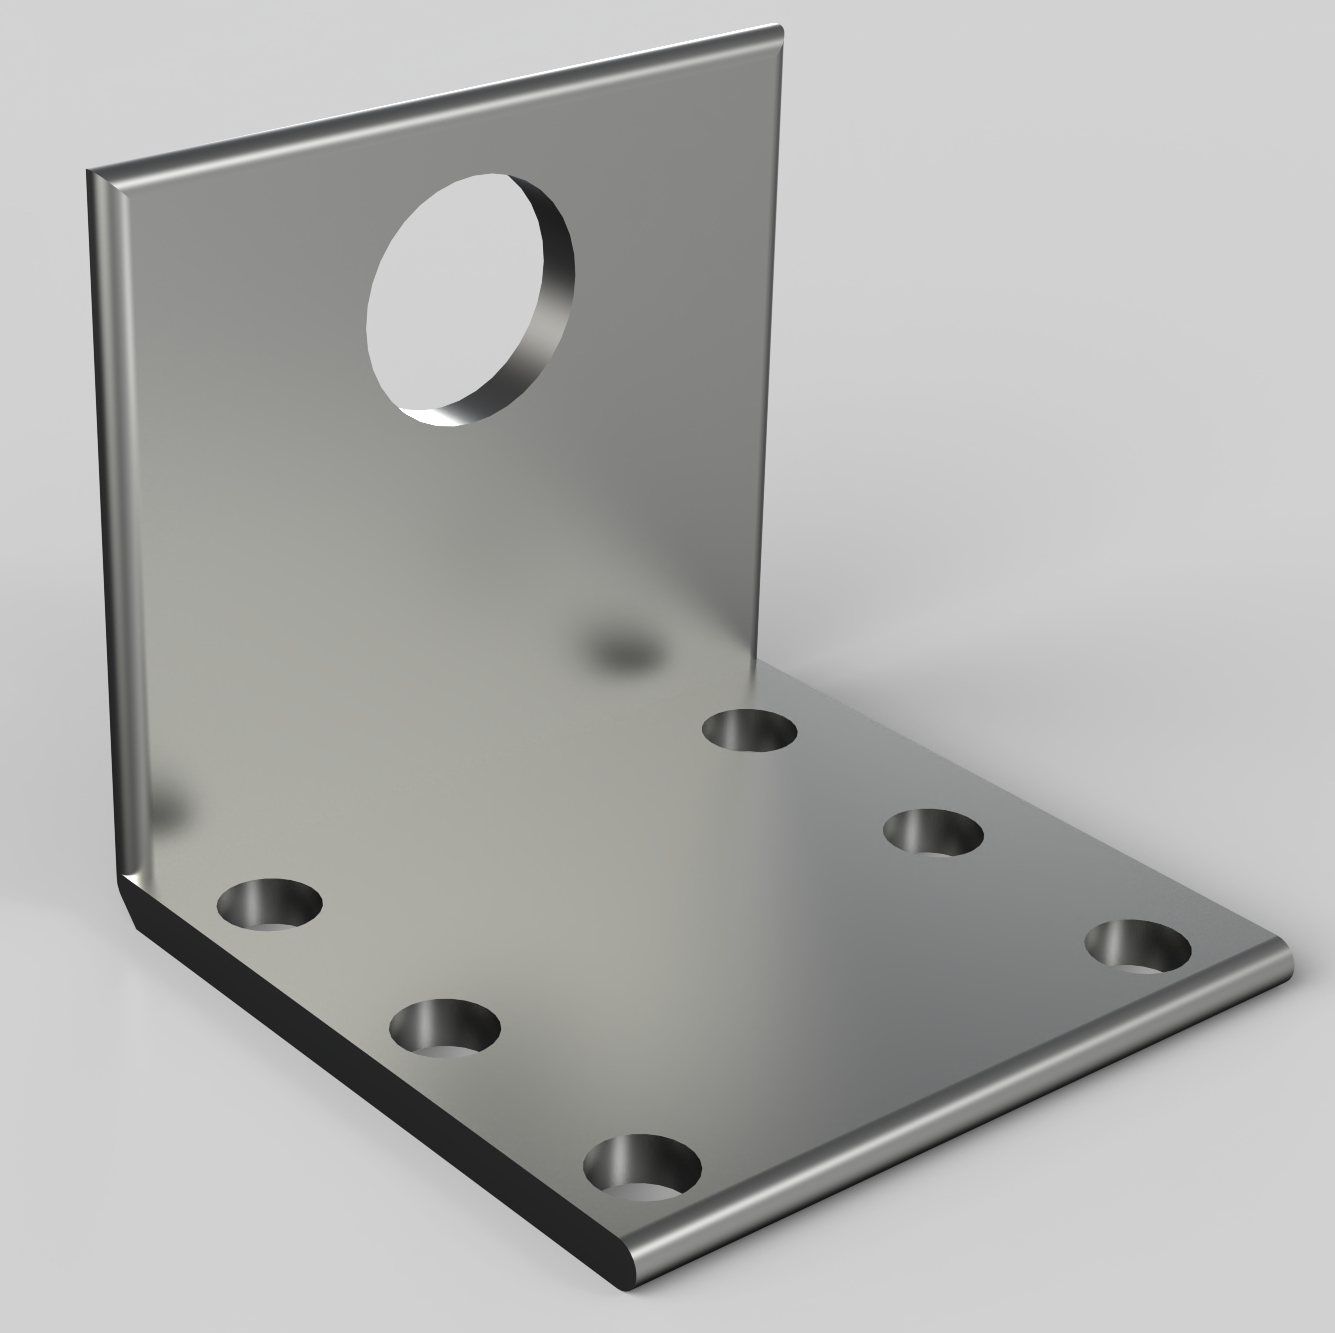
\includegraphics[height=6cm,width=1\textwidth,keepaspectratio]{HW_CAE_STR1_1.png}
                % \caption{caption_name}
                \label{fig:HW_CAE_STR1_1.png}
            \end{figure}
        \end{column}
    \end{columns}
\end{frame}

\begin{frame}[t]{Task 2}
    % \framesubtitle{}
    \vspace{-0.4cm}
    \begin{columns}[T,onlytextwidth]
        \begin{column}{0.59\textwidth}
            \scriptsize
            \textbf{Zip archive, which contains all needed data}: \textit{HWs/HW\_CAE\_STR1/task\_data/HW\_CAE\_STR1\_2.zip}
            \begin{enumerate}
                \item Take the detail from zip archive
                \item You need to create idealized model: remove all edge bending, useless holes. You should cut the object on several pieces for easier mesh creating.
                \item Generate a mesh using hexahedron
                \item Assign <<Aluminum>> material
                \item In simulation constant temperature on the left part of the body is 620$^\circ$. Convection cooling should be on the right side.
                \item Calculate a heat transfer in statics. Compare results, when you assign different materials (brass, steel)
            \end{enumerate}
        \end{column}
        \begin{column}{0.39\textwidth}
            \begin{figure}[H]
                \centering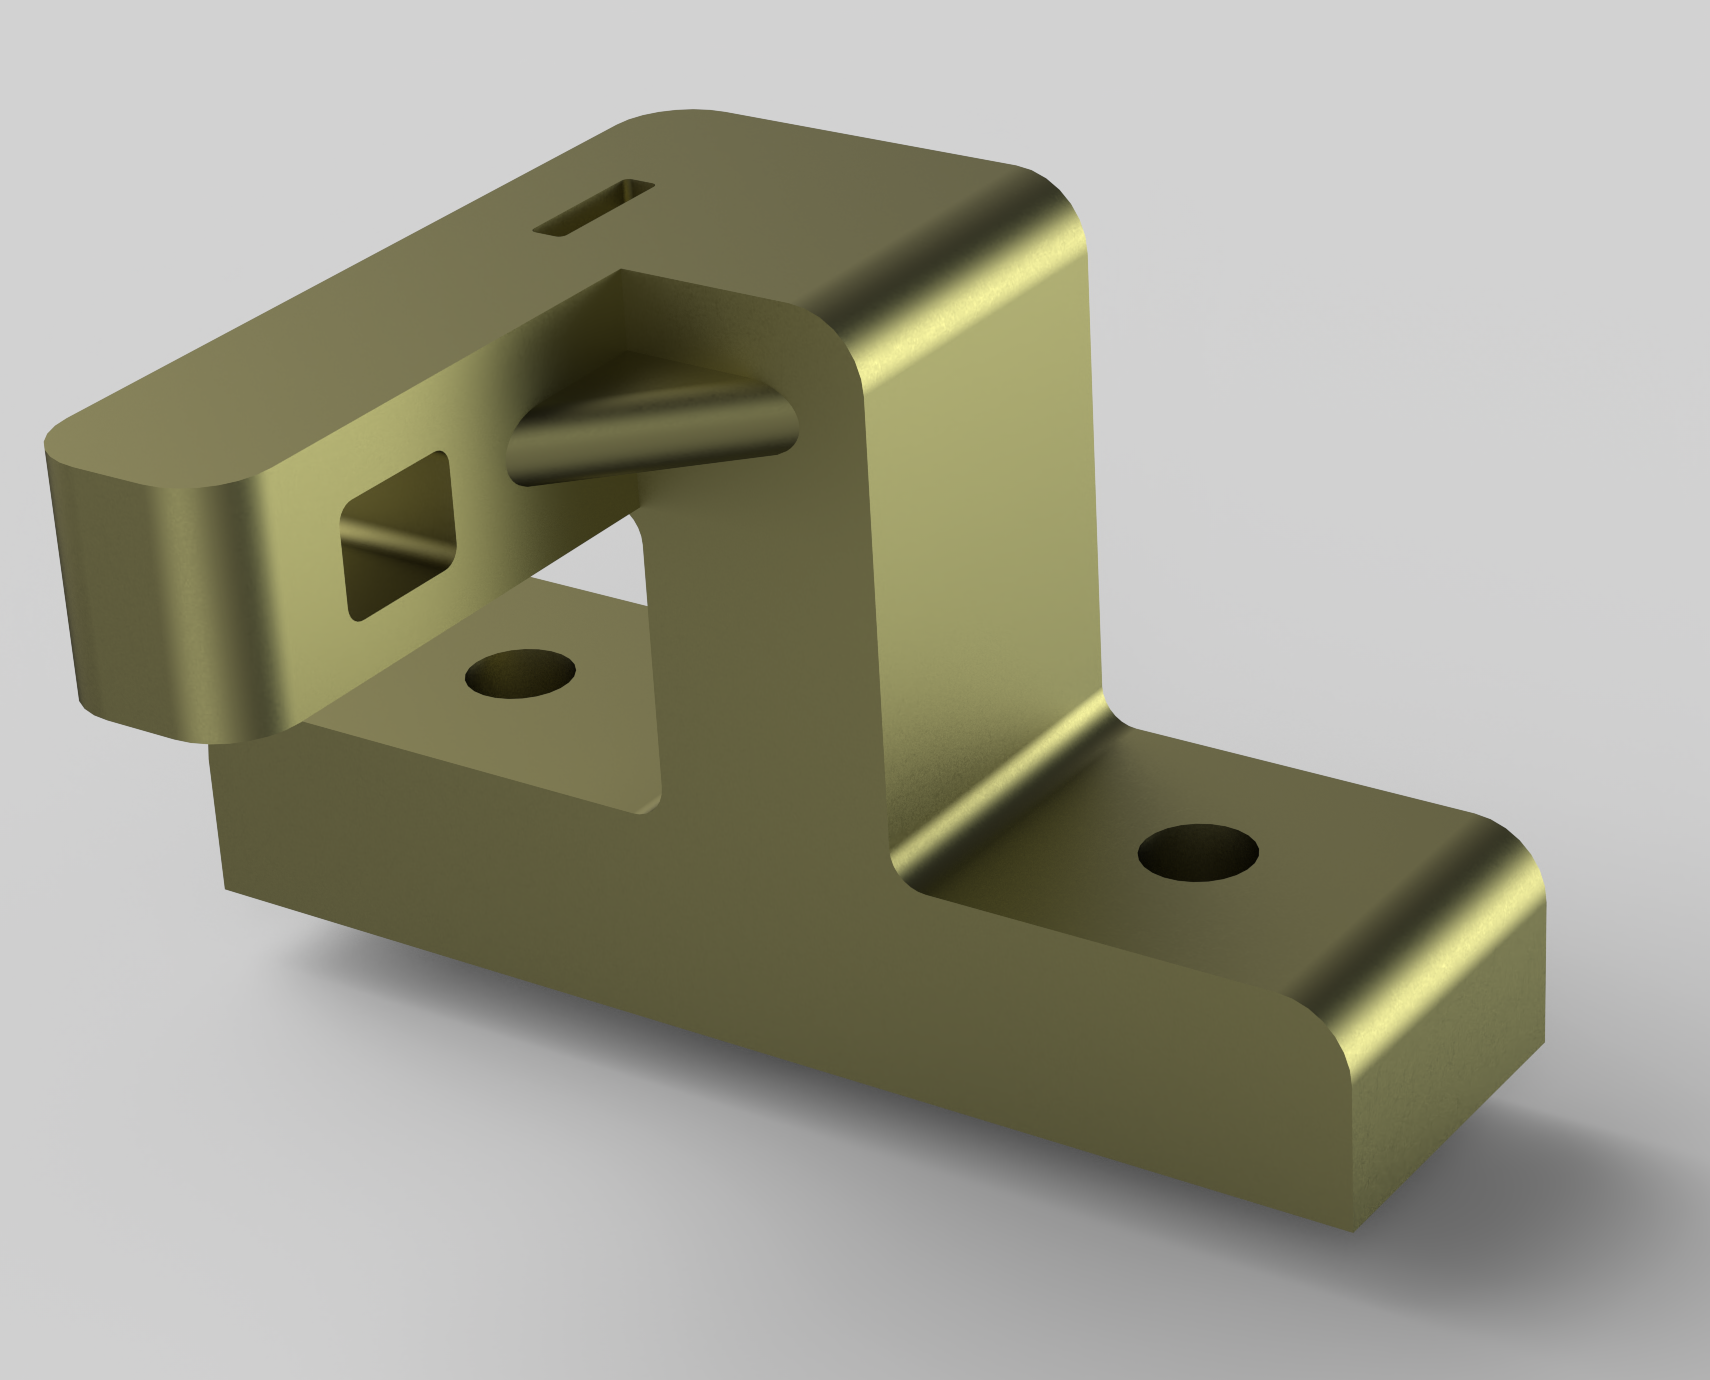
\includegraphics[height=6cm,width=1\textwidth,keepaspectratio]{HW_CAE_STR1_2.png}
                % \caption{caption_name}
                \label{fig:HW_CAE_STR1_2.png}
            \end{figure}
        \end{column}
    \end{columns}
\end{frame}

\begin{frame}[t]{Task 3}
    % \framesubtitle{}
    \vspace{-0.4cm}
    \begin{columns}[T,onlytextwidth]
        \begin{column}{0.59\textwidth}
            \scriptsize
            \textbf{Zip archive, which contains all needed data}: \textit{HWs/HW\_CAE\_STR1/task\_data/HW\_CAE\_STR1\_3.zip}
            \begin{enumerate}
                \item Take the detail from zip archive
                \item Assign <<Aluminum>> material
                \item Find the biggest hole in detail and make a static stress analysis in 2 ways:
                      \begin{itemize}
                        \scriptsize
                          \item Make a steel rod (the same diam as a hole, 500mm length). Apply a force 3000 N to the end of rod.
                          \item * Remove the rod. Apply a moment (you need to calculate it based on knowledge from 1st bullet) (More info in 9th pdf + Advance Sim Инженерный Анализ pdf page 85)
                          
                            \textbf{This task is not affecting on grade.}
                      \end{itemize}
                \item Compare results
            \end{enumerate}
        \end{column}
        \begin{column}{0.39\textwidth}
            \begin{figure}[H]
                \centering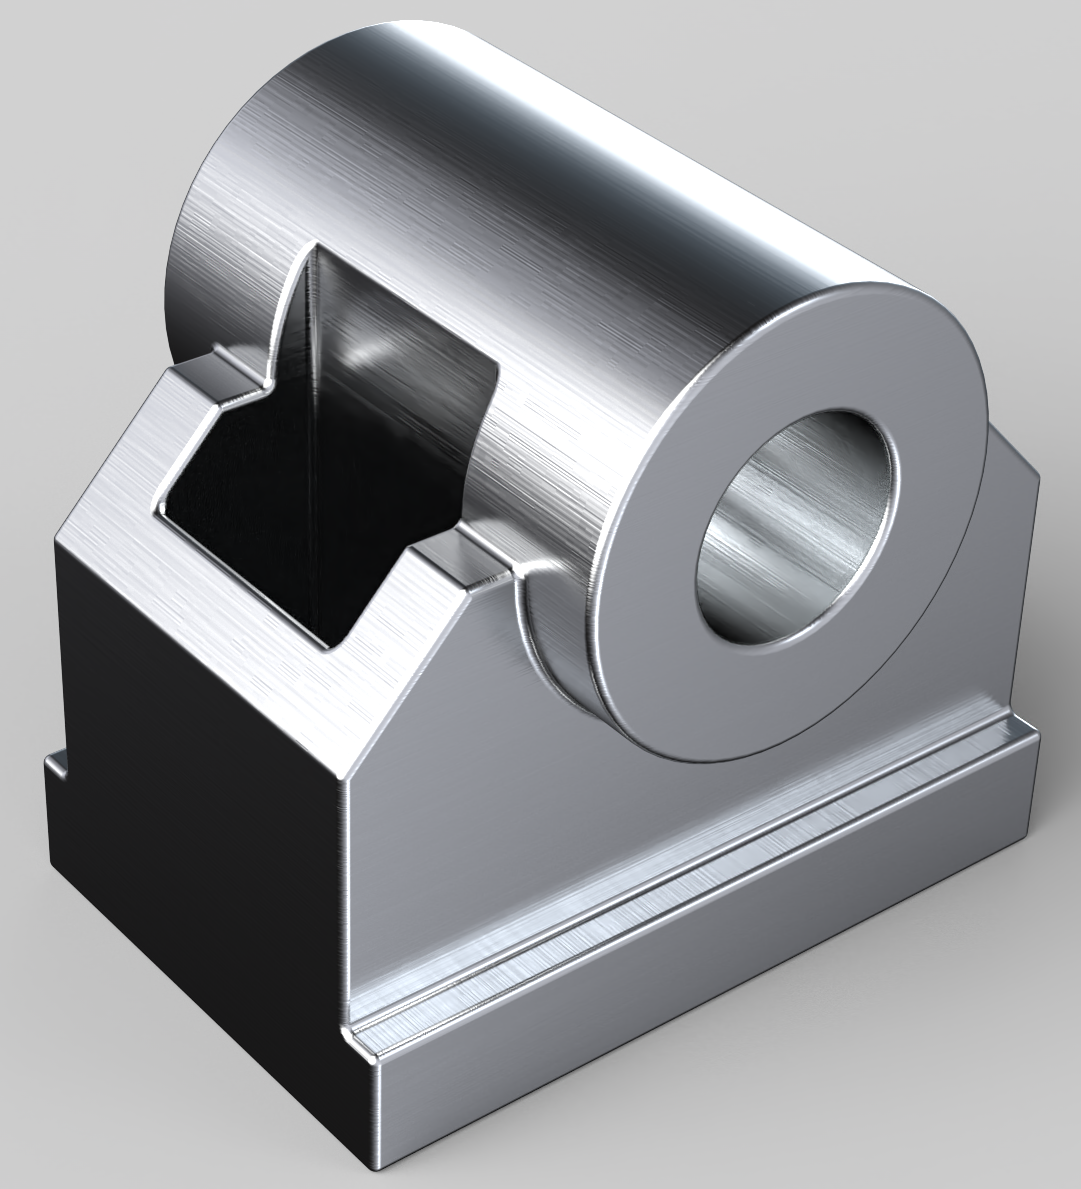
\includegraphics[height=6cm,width=1\textwidth,keepaspectratio]{HW_CAE_STR1_3.png}
                % \caption{caption_name}
                \label{fig:HW_CAE_STR1_3.png}
            \end{figure}
        \end{column}
    \end{columns}
\end{frame}

\begin{frame}[t]{Task 4}
    % \framesubtitle{}
    \vspace{-0.4cm}
    \begin{columns}[T,onlytextwidth]
        \begin{column}{0.54\textwidth}
            \scriptsize
            \textbf{Zip archive, which contains all needed data}: \textit{HWs/HW\_CAE\_STR1/task\_data/HW\_CAE\_STR1\_4.zip}
            \begin{enumerate}
                \item Take the detail from zip archive
                \item Assign <<Steel>> material
                \item Generate a mesh using tetrahedron
                \item Solve the task 1) using bolt connection for lugs and 2) without. Explain the difference
                \item The main goal of the task to apply contact between bodies. You should try: 1) automatic 2) manual contact
                \item Apply pressure 500 MPa to the central beam
                \item Show the possible displacement of pins and the who assembly separately.
            \end{enumerate}
        \end{column}
        \begin{column}{0.45\textwidth}
            \vspace{0.5cm}
            \begin{figure}[H]
                \centering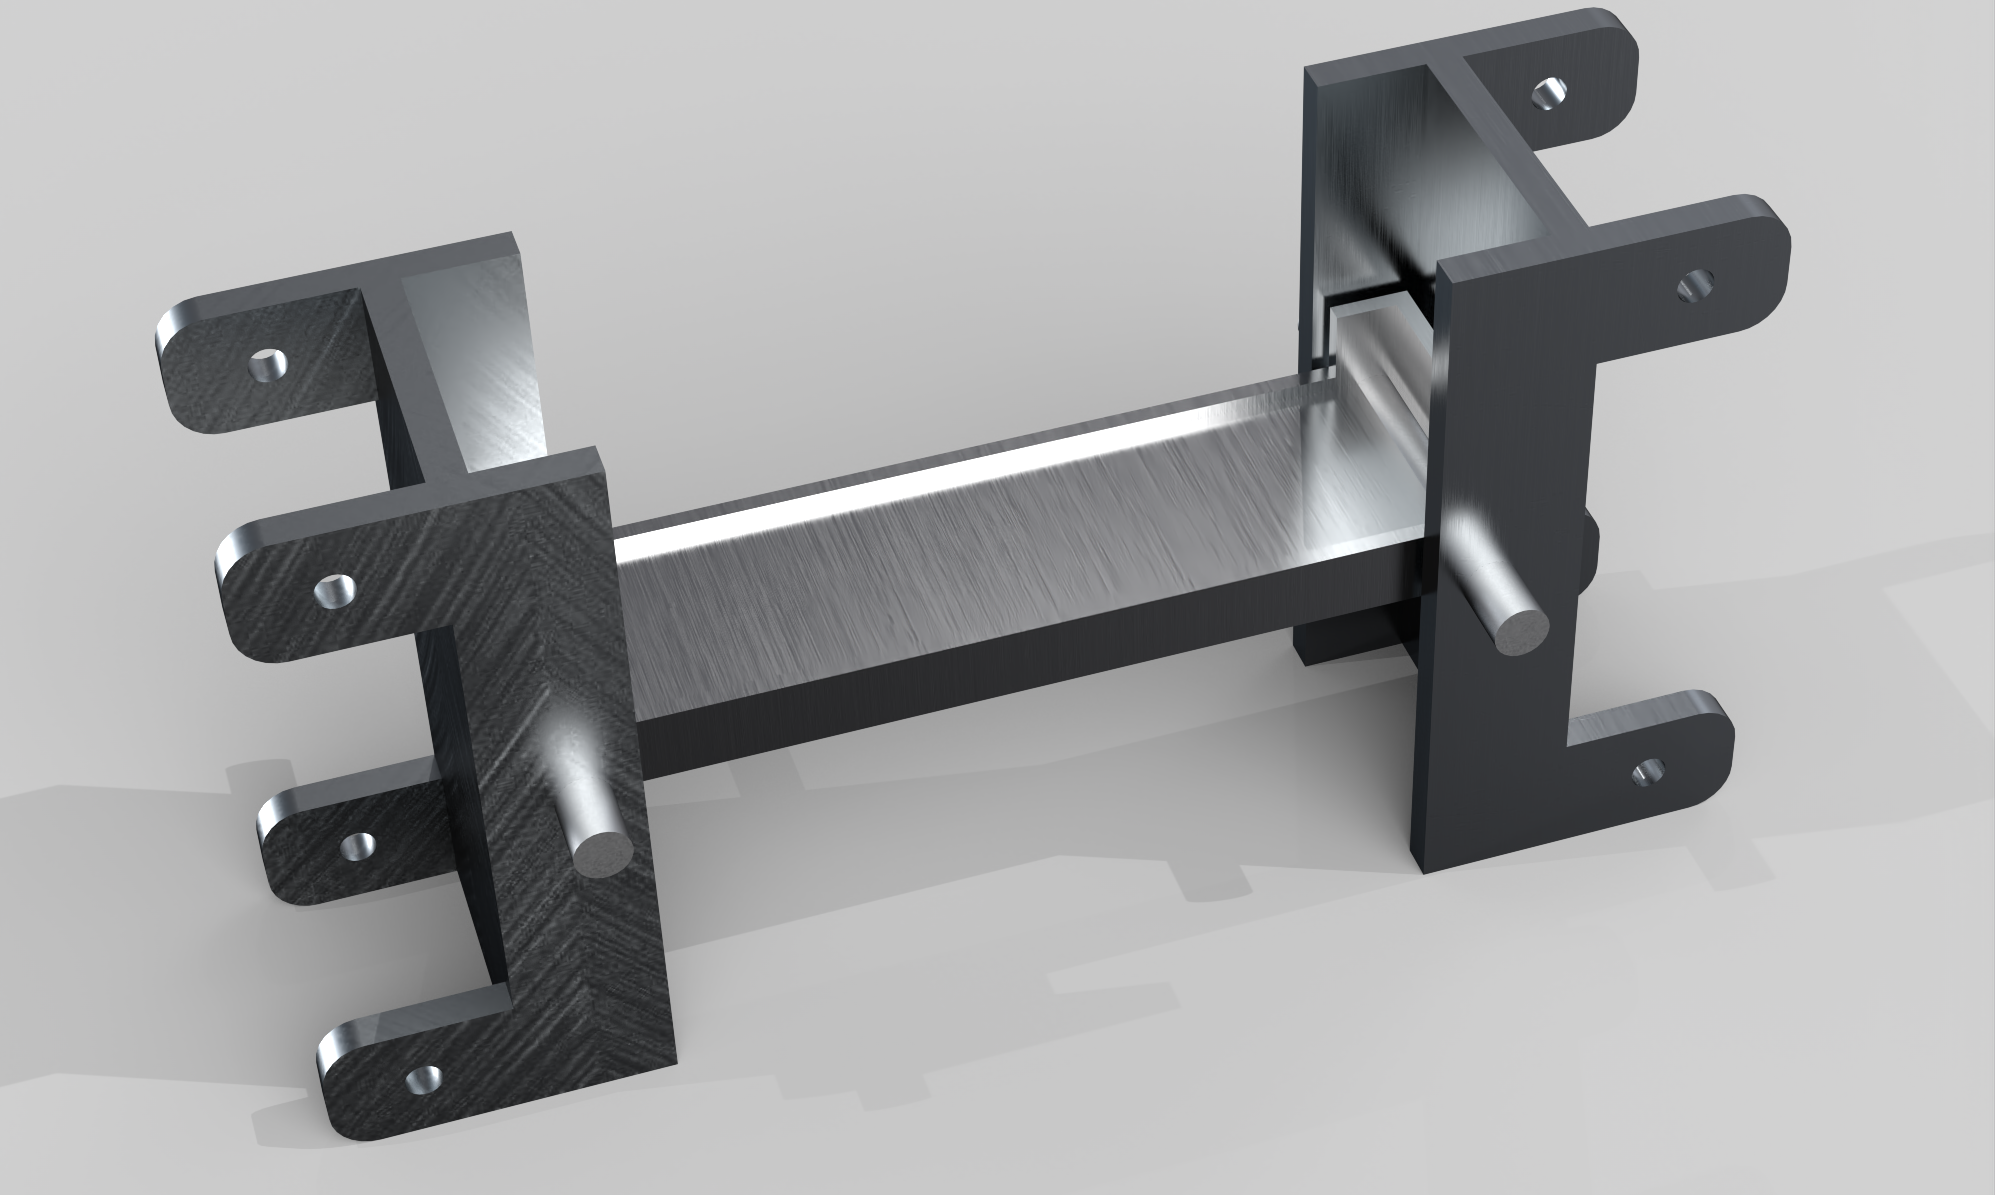
\includegraphics[height=6cm,width=1\textwidth,keepaspectratio]{HW_CAE_STR1_4.png}
                % \caption{caption_name}
                \label{fig:HW_CAE_STR1_4.png}
            \end{figure}
        \end{column}
    \end{columns}
\end{frame}

\fbckg{fibeamer/figs/last_page.png}
\frame[plain]{}

\end{document}